\chapter{Development}~\label{cha:development}
Development of the application was divided into two main parts: the frontend and the backend, with the backend further broken up into its constituent services. The entire project was maintained in a single mono-repository, with each backend service and the frontend housed in separate directories. While this is not necessarily the optimal structure for a larger project this approach reduced overhead for a project of smaller scope, making it the most practical solution.

\section{Frontend}~\label{sec:frontend-development}
\subsection{Implementation}
The actual implementation of the frontend used Vite as a development server and build tool for the React frontend. This gave a starting TypeScript template which was modified to create the application.

Once the build system was in place the design was broken up so that each component could be built independently. The HeroUI component library used in this project provided basic components common to most web applications, such as buttons, modals, and input fields from these the more complex components could be built. One of the benefits of using this component library was its integration with Tailwind CSS, which allowed for stylings to be applied through class names rather than bespoke stylesheets. This greatly reduced the amount of time needed to style the application and ensured a consistent look across the application.

After completing the frontend components, the next step was to integrate them with the backend services. Some functionalities required user authentication through Spotify to access key Spotify API features. This had to be implemented on the frontend using Spotify’s OAuth2 flow, which redirects the user to Spotify for login and then returns them to the application with an access token in the URL which is read by the application and saved to local storage, so sessions persist between refreshes.

Once the authentication was implemented, the remaining backend API endpoints were integrated using the Axios library, allowing the frontend to communicate efficiently with the various services.

Once the authentication was implemented, all remaining endpoint calls were implemented as functions that can be imported and run by any component. This was done using the Axios library, which though not a native JavaScript library, is widely used and well documented which made it easy to implement.

\subsubsection{Landing Page}
An oversight in the original design was the lack of a landing page which is presented to users before logging. The page follows the stylings of the application and contains graphics and text related to the application. Once the user logs in they are redirected to the scan screen.

\begin{figure} [H]
    \centering
    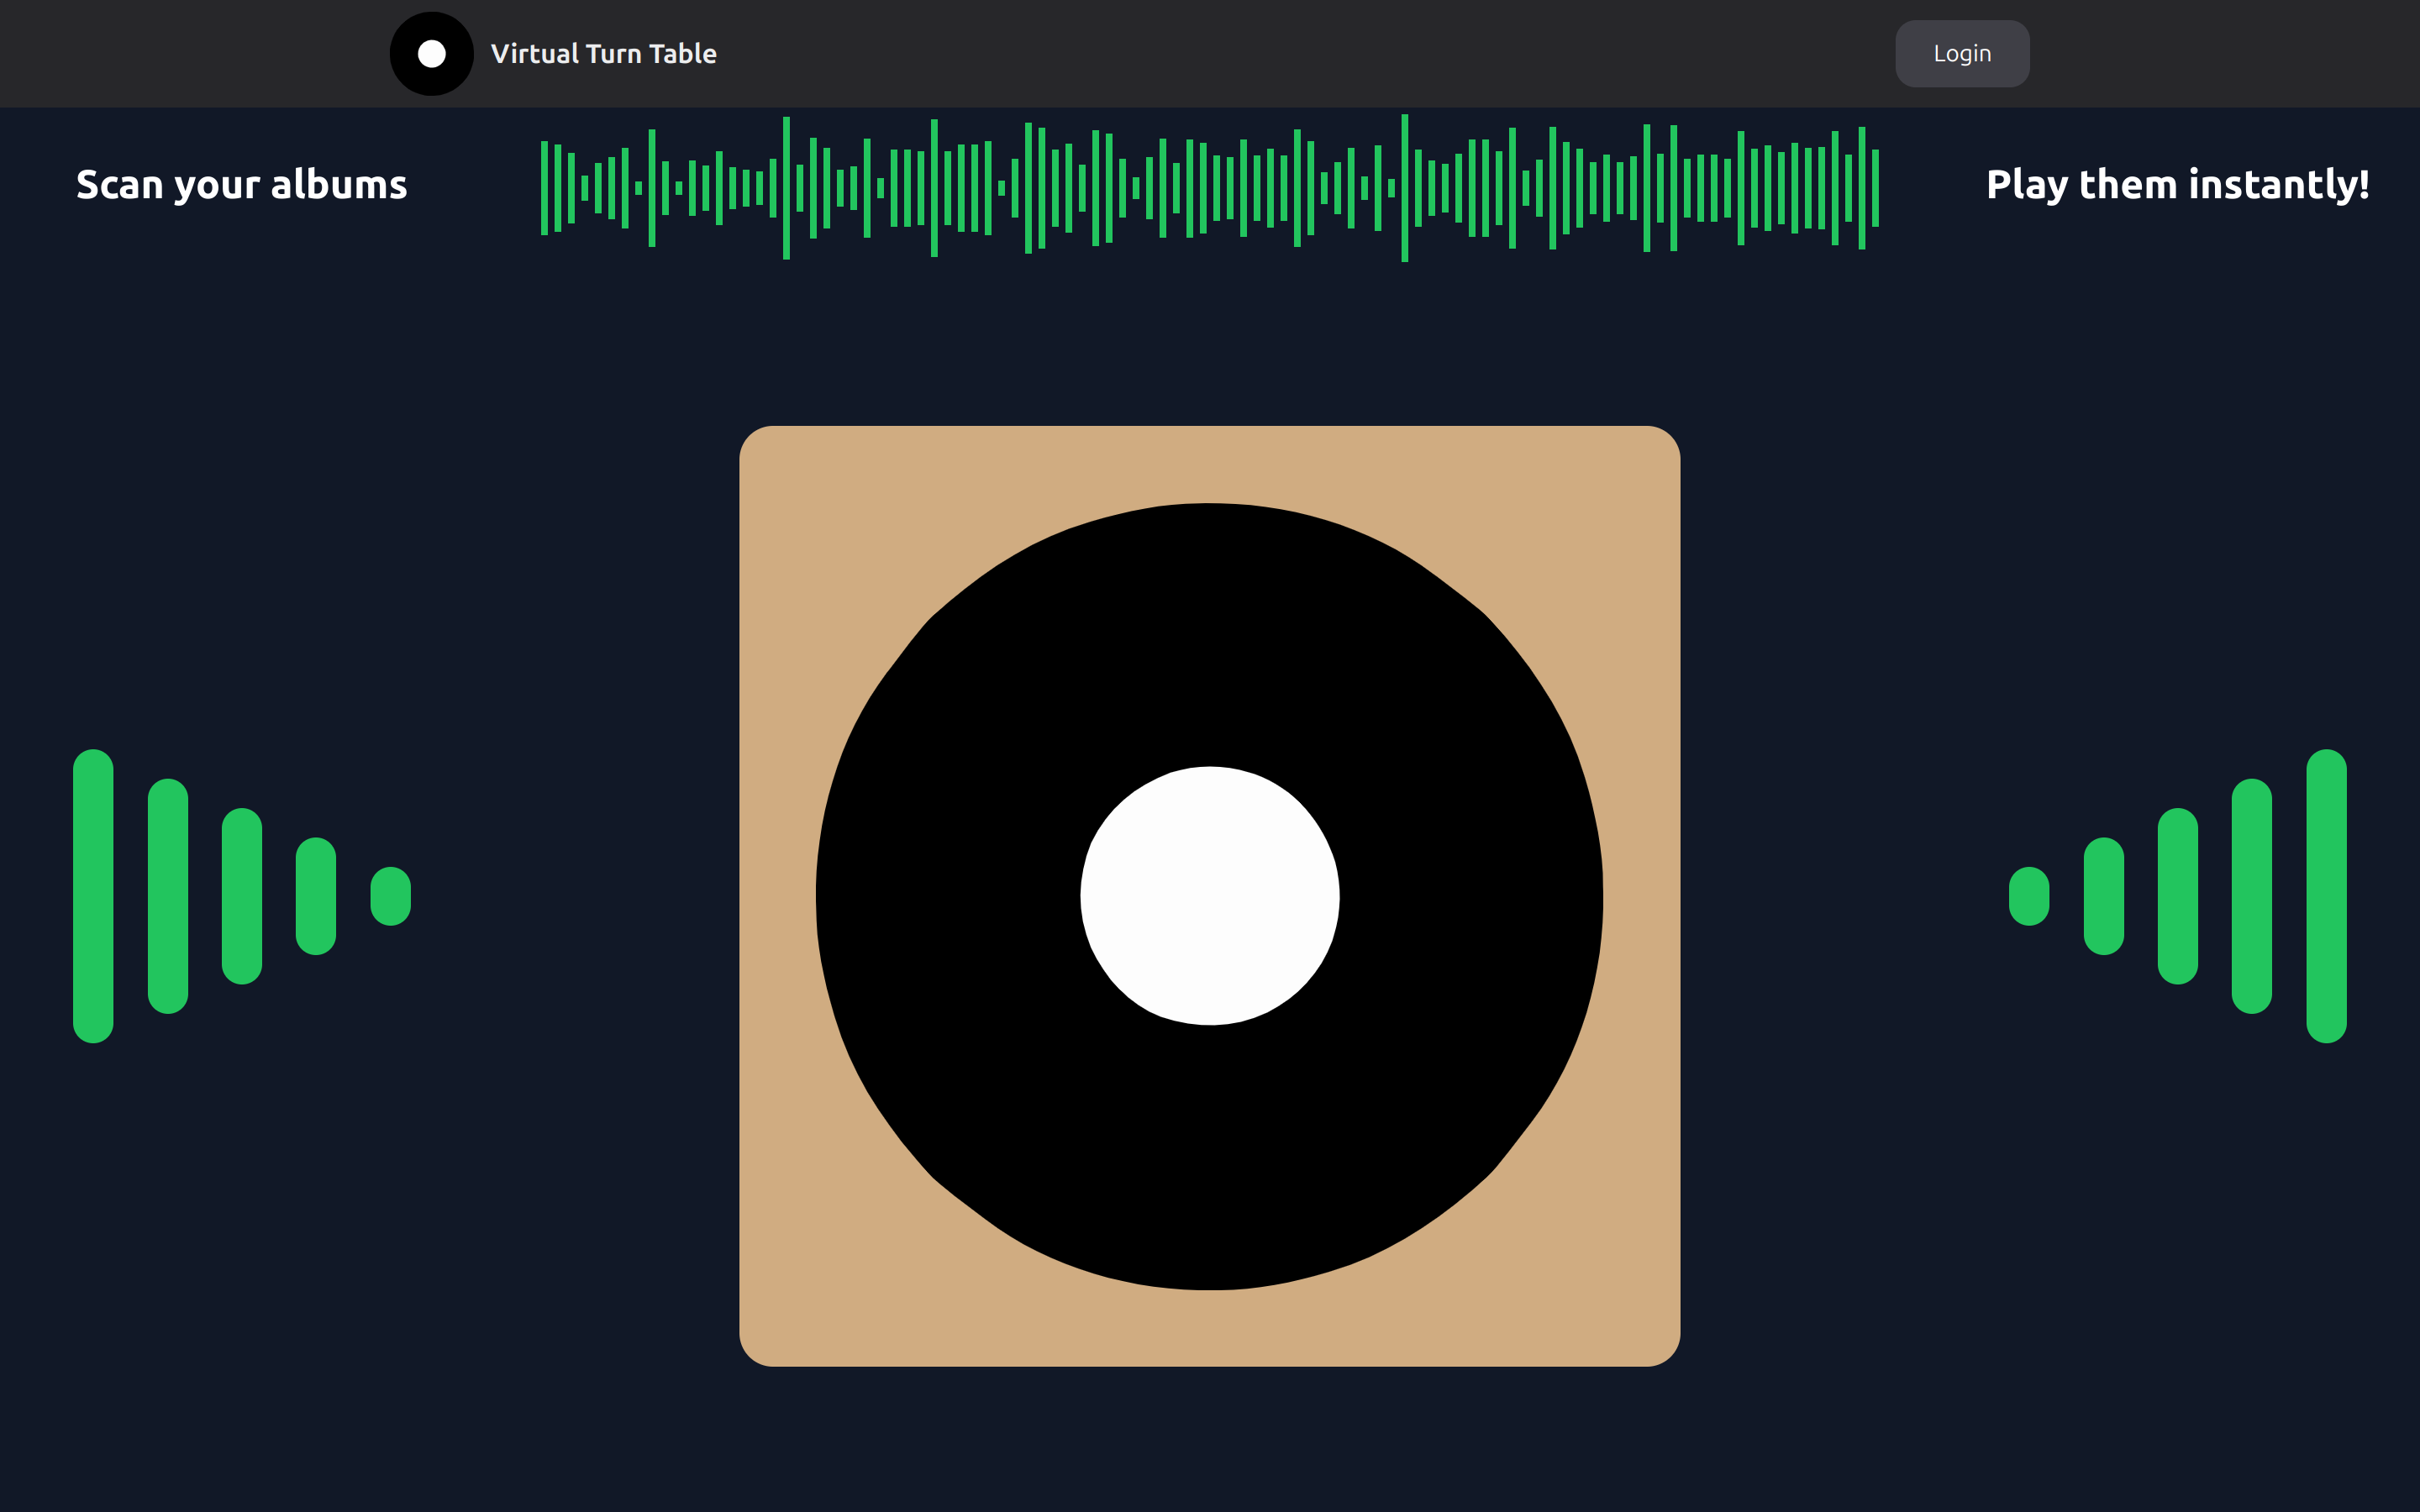
\includegraphics[width=0.8\textwidth]{figures/landing_page.png}
    \caption{The landing page of the application}
    \label{fig:landing_page}
\end{figure}


\subsubsection{Navigation Bar}
The navigation bar is a component included on all screens which allows the user to navigate between the different screens of the application. It consists of a static logo, screen selection tabs, and user details. The user details also serves as a dropdown trigger which displays a menu, as seen in Figure~\ref{fig:user_options_menu}, with account options such as setting their collection to public, sharing their collection with a certain user, deleting their account, and logging out.

\begin{figure} [H]
    \centering
    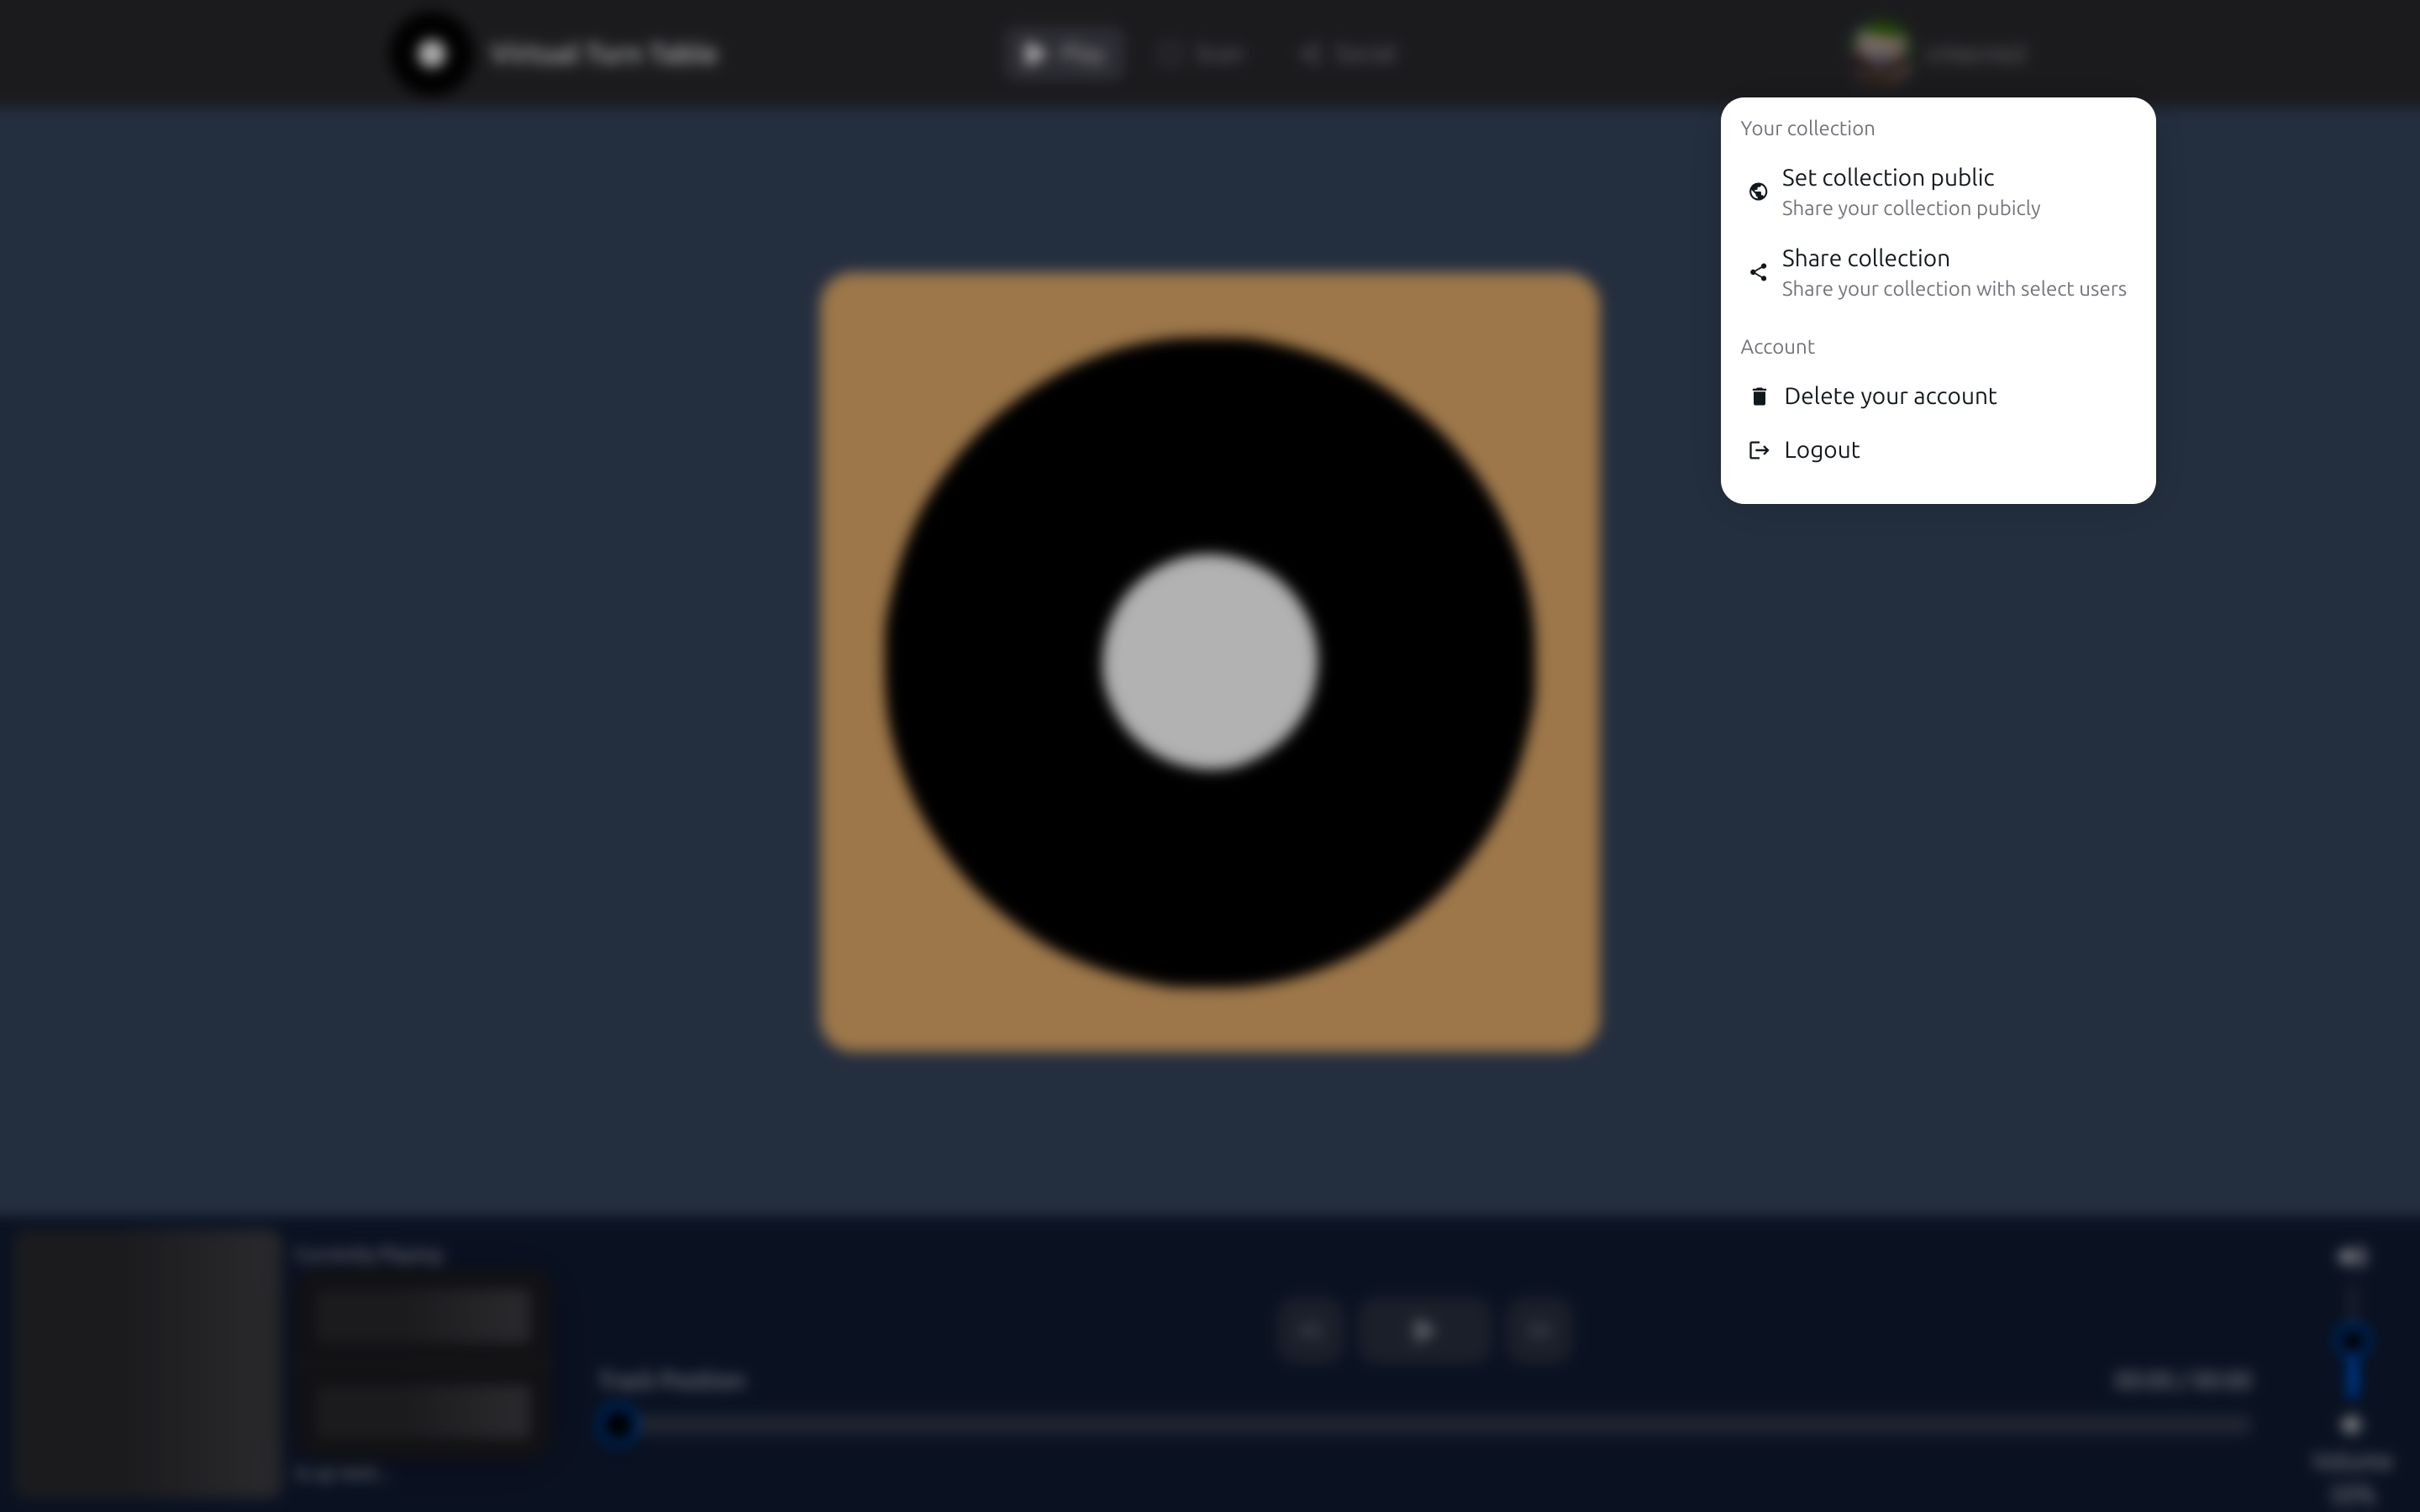
\includegraphics[width=0.8\textwidth]{figures/menu_open_screen.png}
    \caption{The user options menu opened from the navigation bar}
    \label{fig:user_options_menu}
\end{figure}

\subsubsection{Play Screen}
The play screen largely follows the initial design, consisting of three main sections: the track list, the controls, and a spinning vinyl animation. Music playback is handled by the Spotify Web Playback SDK, a client side JavaScript library that enables real-time control of Spotify playback within the browser. Actions such as changing tracks, skipping forward or backward, and pausing are executed by invoking the corresponding methods provided by the SDK.

\paragraph{Track List}
The track list displays all tracks from the currently active album, which is set on the scan screen. It serves as a selection menu of tracks, allowing users to choose a specific song for playback similarly to a music streaming service. The component is styled to fill up all vertical space between the navigation bar and scrolls vertically if the number of tracks exceeds the available space.

\paragraph{Controls}
The playback controls consist of buttons and sliders which users can interact with to effect audio playback. Clicking a button or adjusting a slider calls the relevant SDK methods, allowing users to play, pause, skip, or adjust volume. Album art and track information are displayed, so the currently playing track can be easily identified, these automatically update as the active song changes.
One feature from the original design was removed, the ability to scrub through the whole album rather than only the currently playing track. This was considered too complex to implement and added little to the user experience and so was excluded from the final implementation.

\paragraph{Spinning Vinyl}
To emulate the feel of a physical record player, an animated spinning vinyl graphic was implemented, featuring the album cover in the centre. Just as if this were a real record player, the vinyl rotates when music is playing and stops when paused. This was controlled by editing the rotation styling of the graphic.

A second animation was added to simulate the act of removing the vinyl from its sleeve when changing albums. This is meant to replicate the experience of removing a vinyl record from its sleeve and placing it on the turntable. This was done by animating the vinyl graphic to move to the side of the screen and then back to the centre with a new album cover.

\begin{figure} [H]
    \centering
    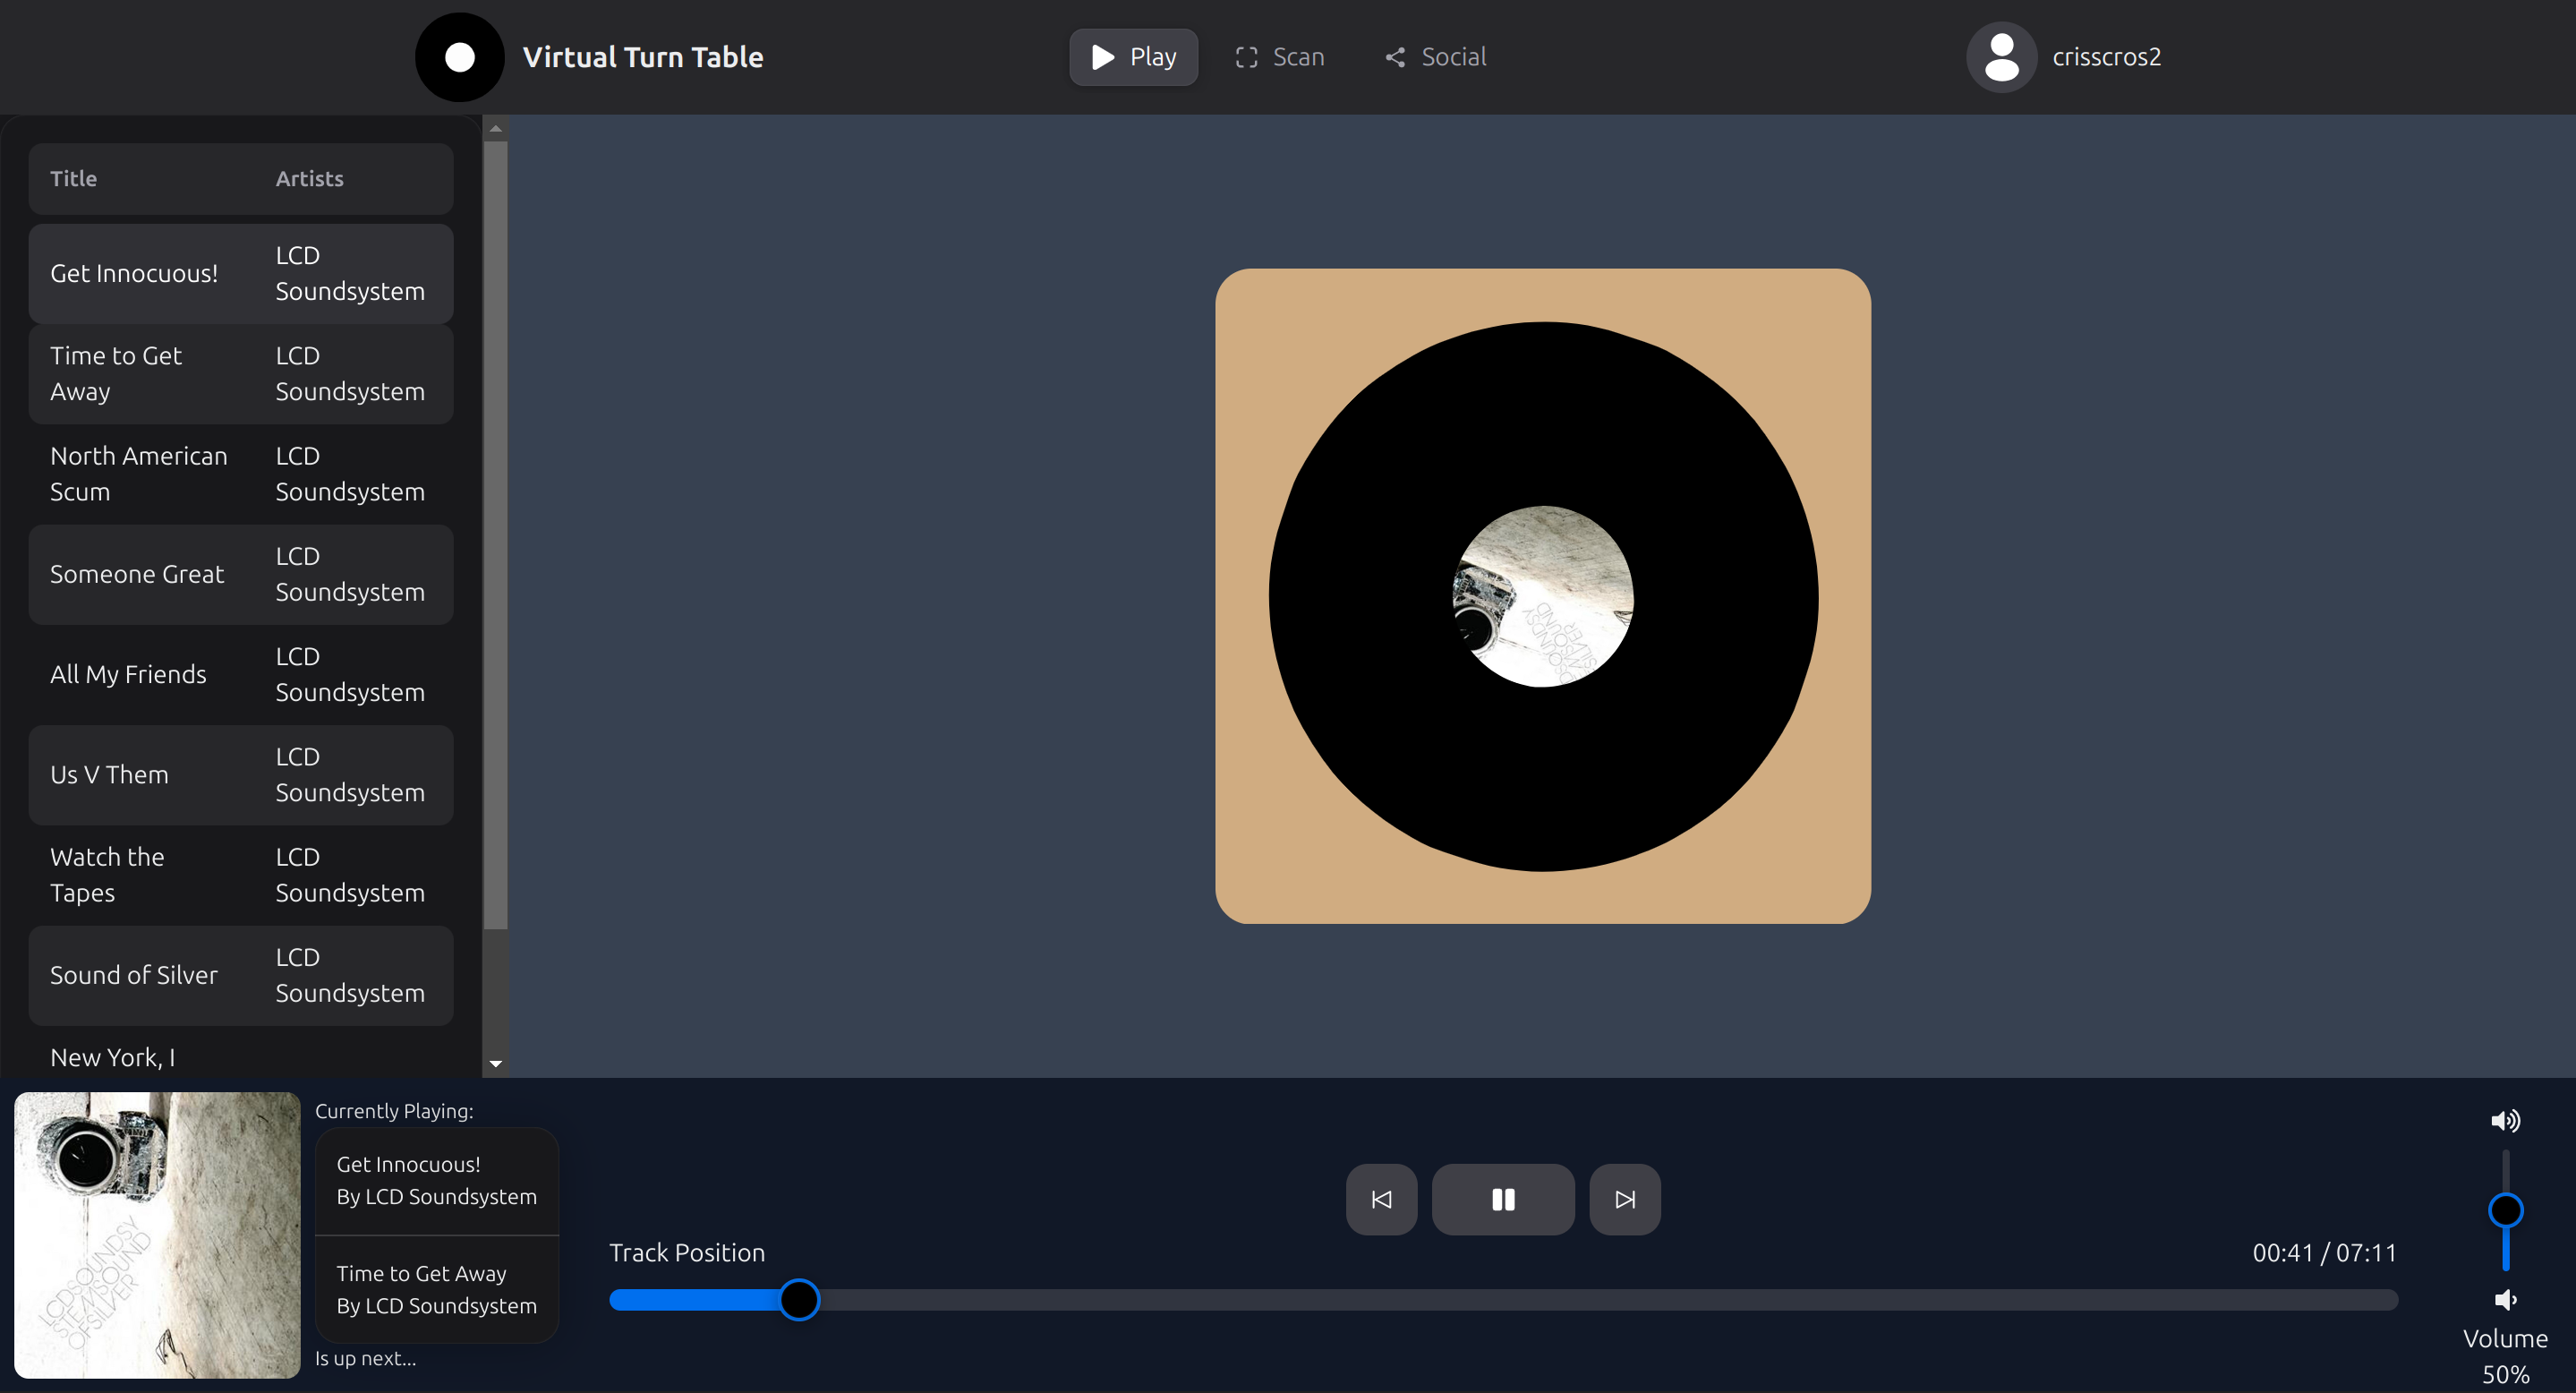
\includegraphics[width=0.8\textwidth]{figures/play_screen.png}
    \caption{The play screen of the application}
    \label{fig:play_screen}
\end{figure}

\subsubsection{Scan Screen}
The scan screen, though following the initial design as closely as possible, had to be changed during development as some problems with the original design became clear. It was also split into three main parts like the play screen: the album confirmation sidebar, the scan section, and the album collection.

\paragraph{Album Confirmation Sidebar}
The album confirmation sidebar existed to allow the user to confirm the album that was guessed was the correct one. This presented a problem that was not considered in the original design, what if the album guessed was incorrect? To solve this a second stage of the confirmation with a separate scatter shot approach taken to find the correct album which can be seen in Figure~\ref{fig:album_confirmation_sidebar_incorrect}. The sidebar also acts as a way to show to the user the application is processing as whilst the application is determining the album the sidebar is animated to show a loading animation providing feedback to the user that the application has not broken. Once the user confirms the album selection the sidebar slides back to the side of the screen and the album is set as the active album.

\begin{figure}[H]
    \centering
    \begin{subfigure}[t]{0.3\textwidth}
        \centering
        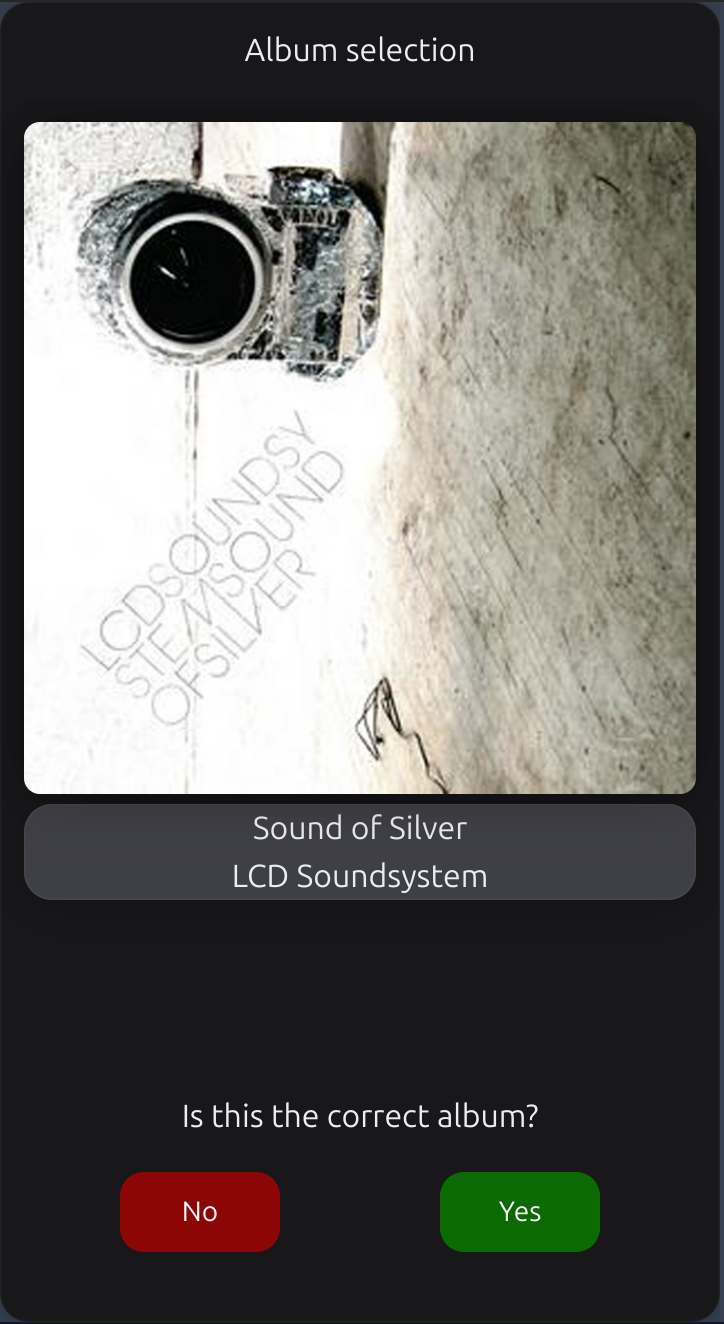
\includegraphics[width=0.8\textwidth]{figures/corrent_album_confirm.png}
        \caption{The album confirmation sidebar with the correct album guessed}
        \label{fig:album_confirmation_sidebar}
    \end{subfigure}
    \begin{subfigure}[t]{0.3\textwidth}
        \centering
        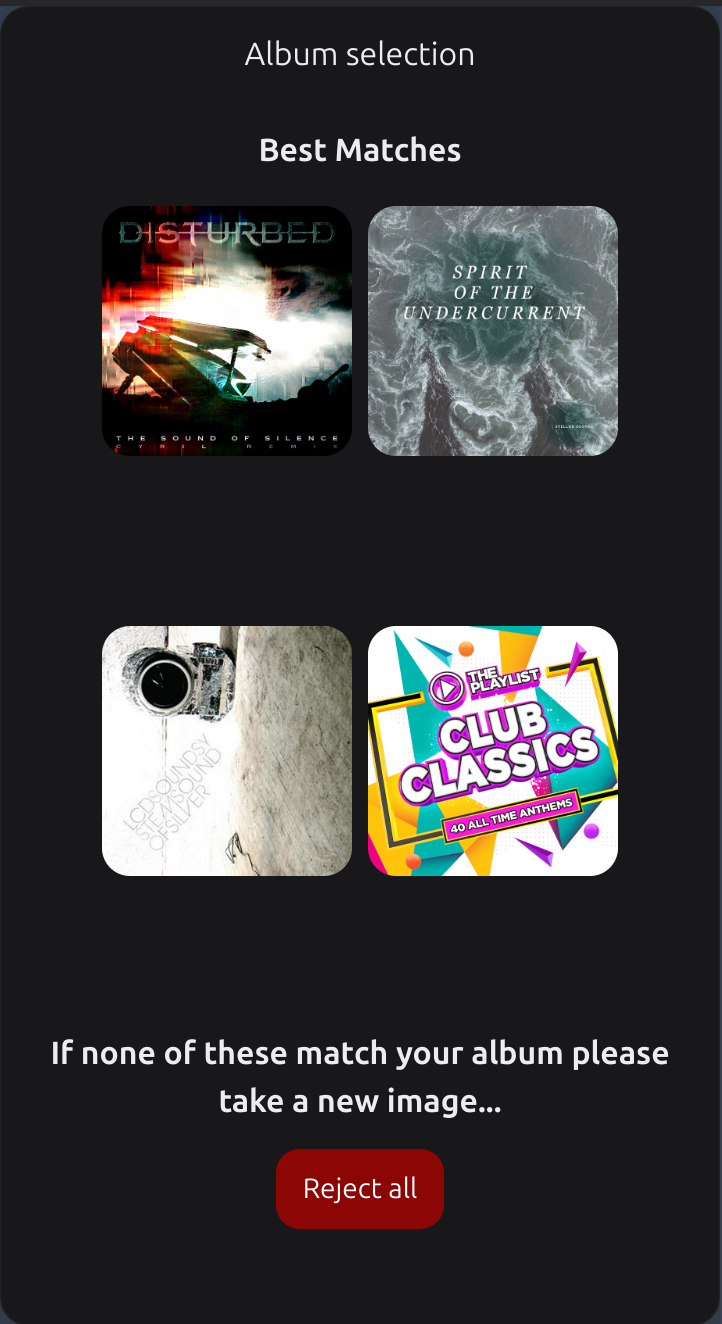
\includegraphics[width=0.8\textwidth]{figures/top_results_confirm.png}
        \caption{The album confirmation sidebar with the incorrect album guessed}
        \label{fig:album_confirmation_sidebar_incorrect}
    \end{subfigure}
\end{figure}

\paragraph{Scan Section}
Similarly to the confirmation sidebar an issue was found with the scan section. The original design did not take into account users who may not have a camera connected to their device. To solve this a file upload, which can be seen in Figure~\ref{fig:upload_component}, was added to the scan section which is the default if no cameras can be accessed by the browser. This could also be accessed if the user did not want to use their camera for any reason.

\begin{figure} [H]
    \centering
    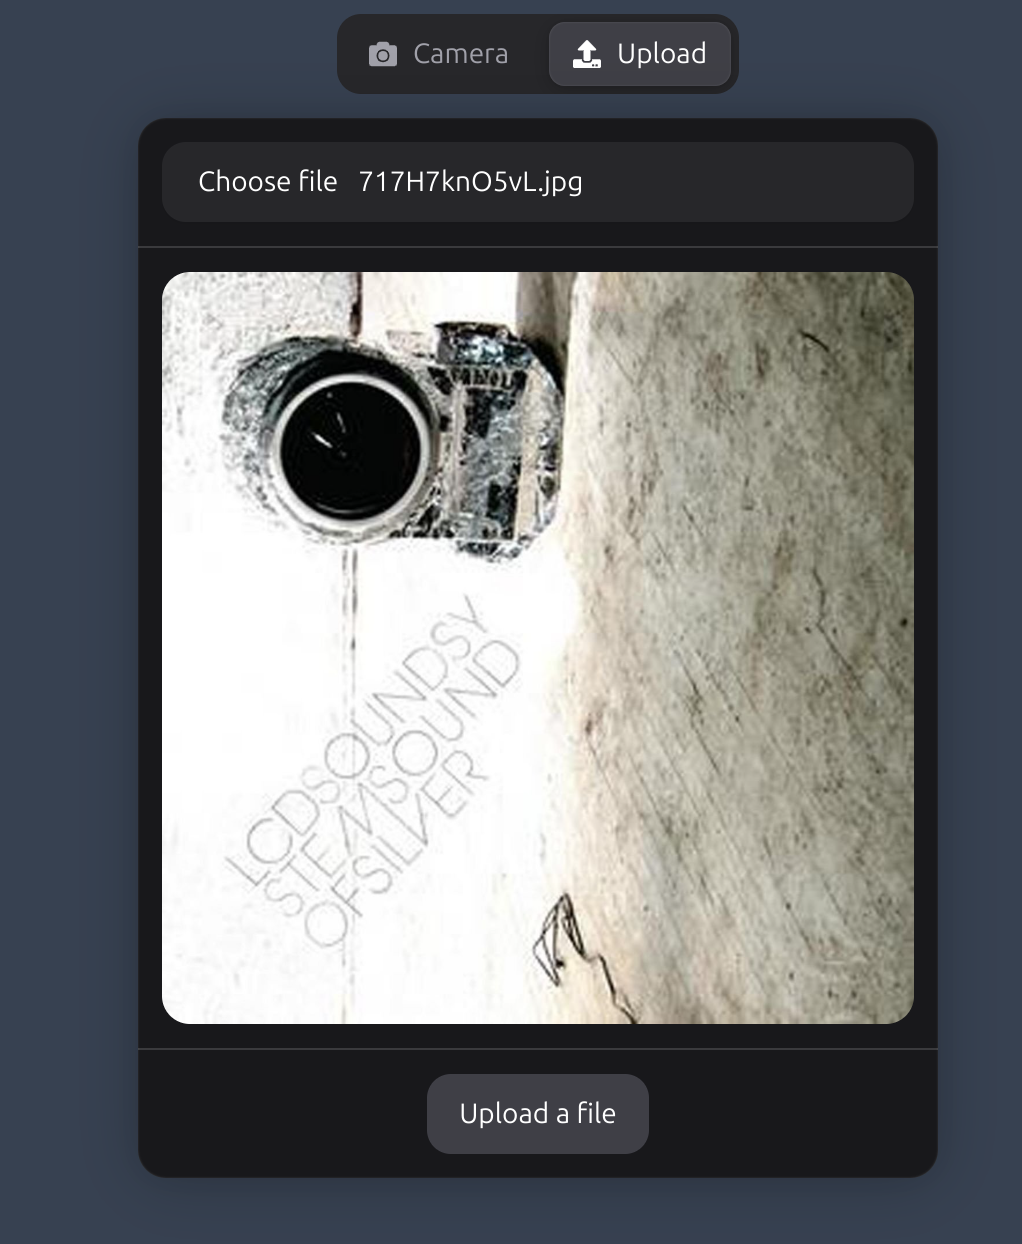
\includegraphics[width=0.4\textwidth]{figures/upload_component.png}
    \caption{The file upload component}
    \label{fig:upload_component}
\end{figure}

\paragraph{Album Collection}
This section of the screen was mostly unchanged from the original design. The user's albums slide across the bottom of the screen and the user can select an album to play by clicking on it. Once the user hovers over an album art the sliding is paused and extra details of that album appear such as the title and artist. The option to look through the user's collection differently is also available by clicking the view all button which opens a modal with all the user's albums in a view reminiscent of flicking through vinyl records in a record store.

\begin{figure} [H]
    \centering
    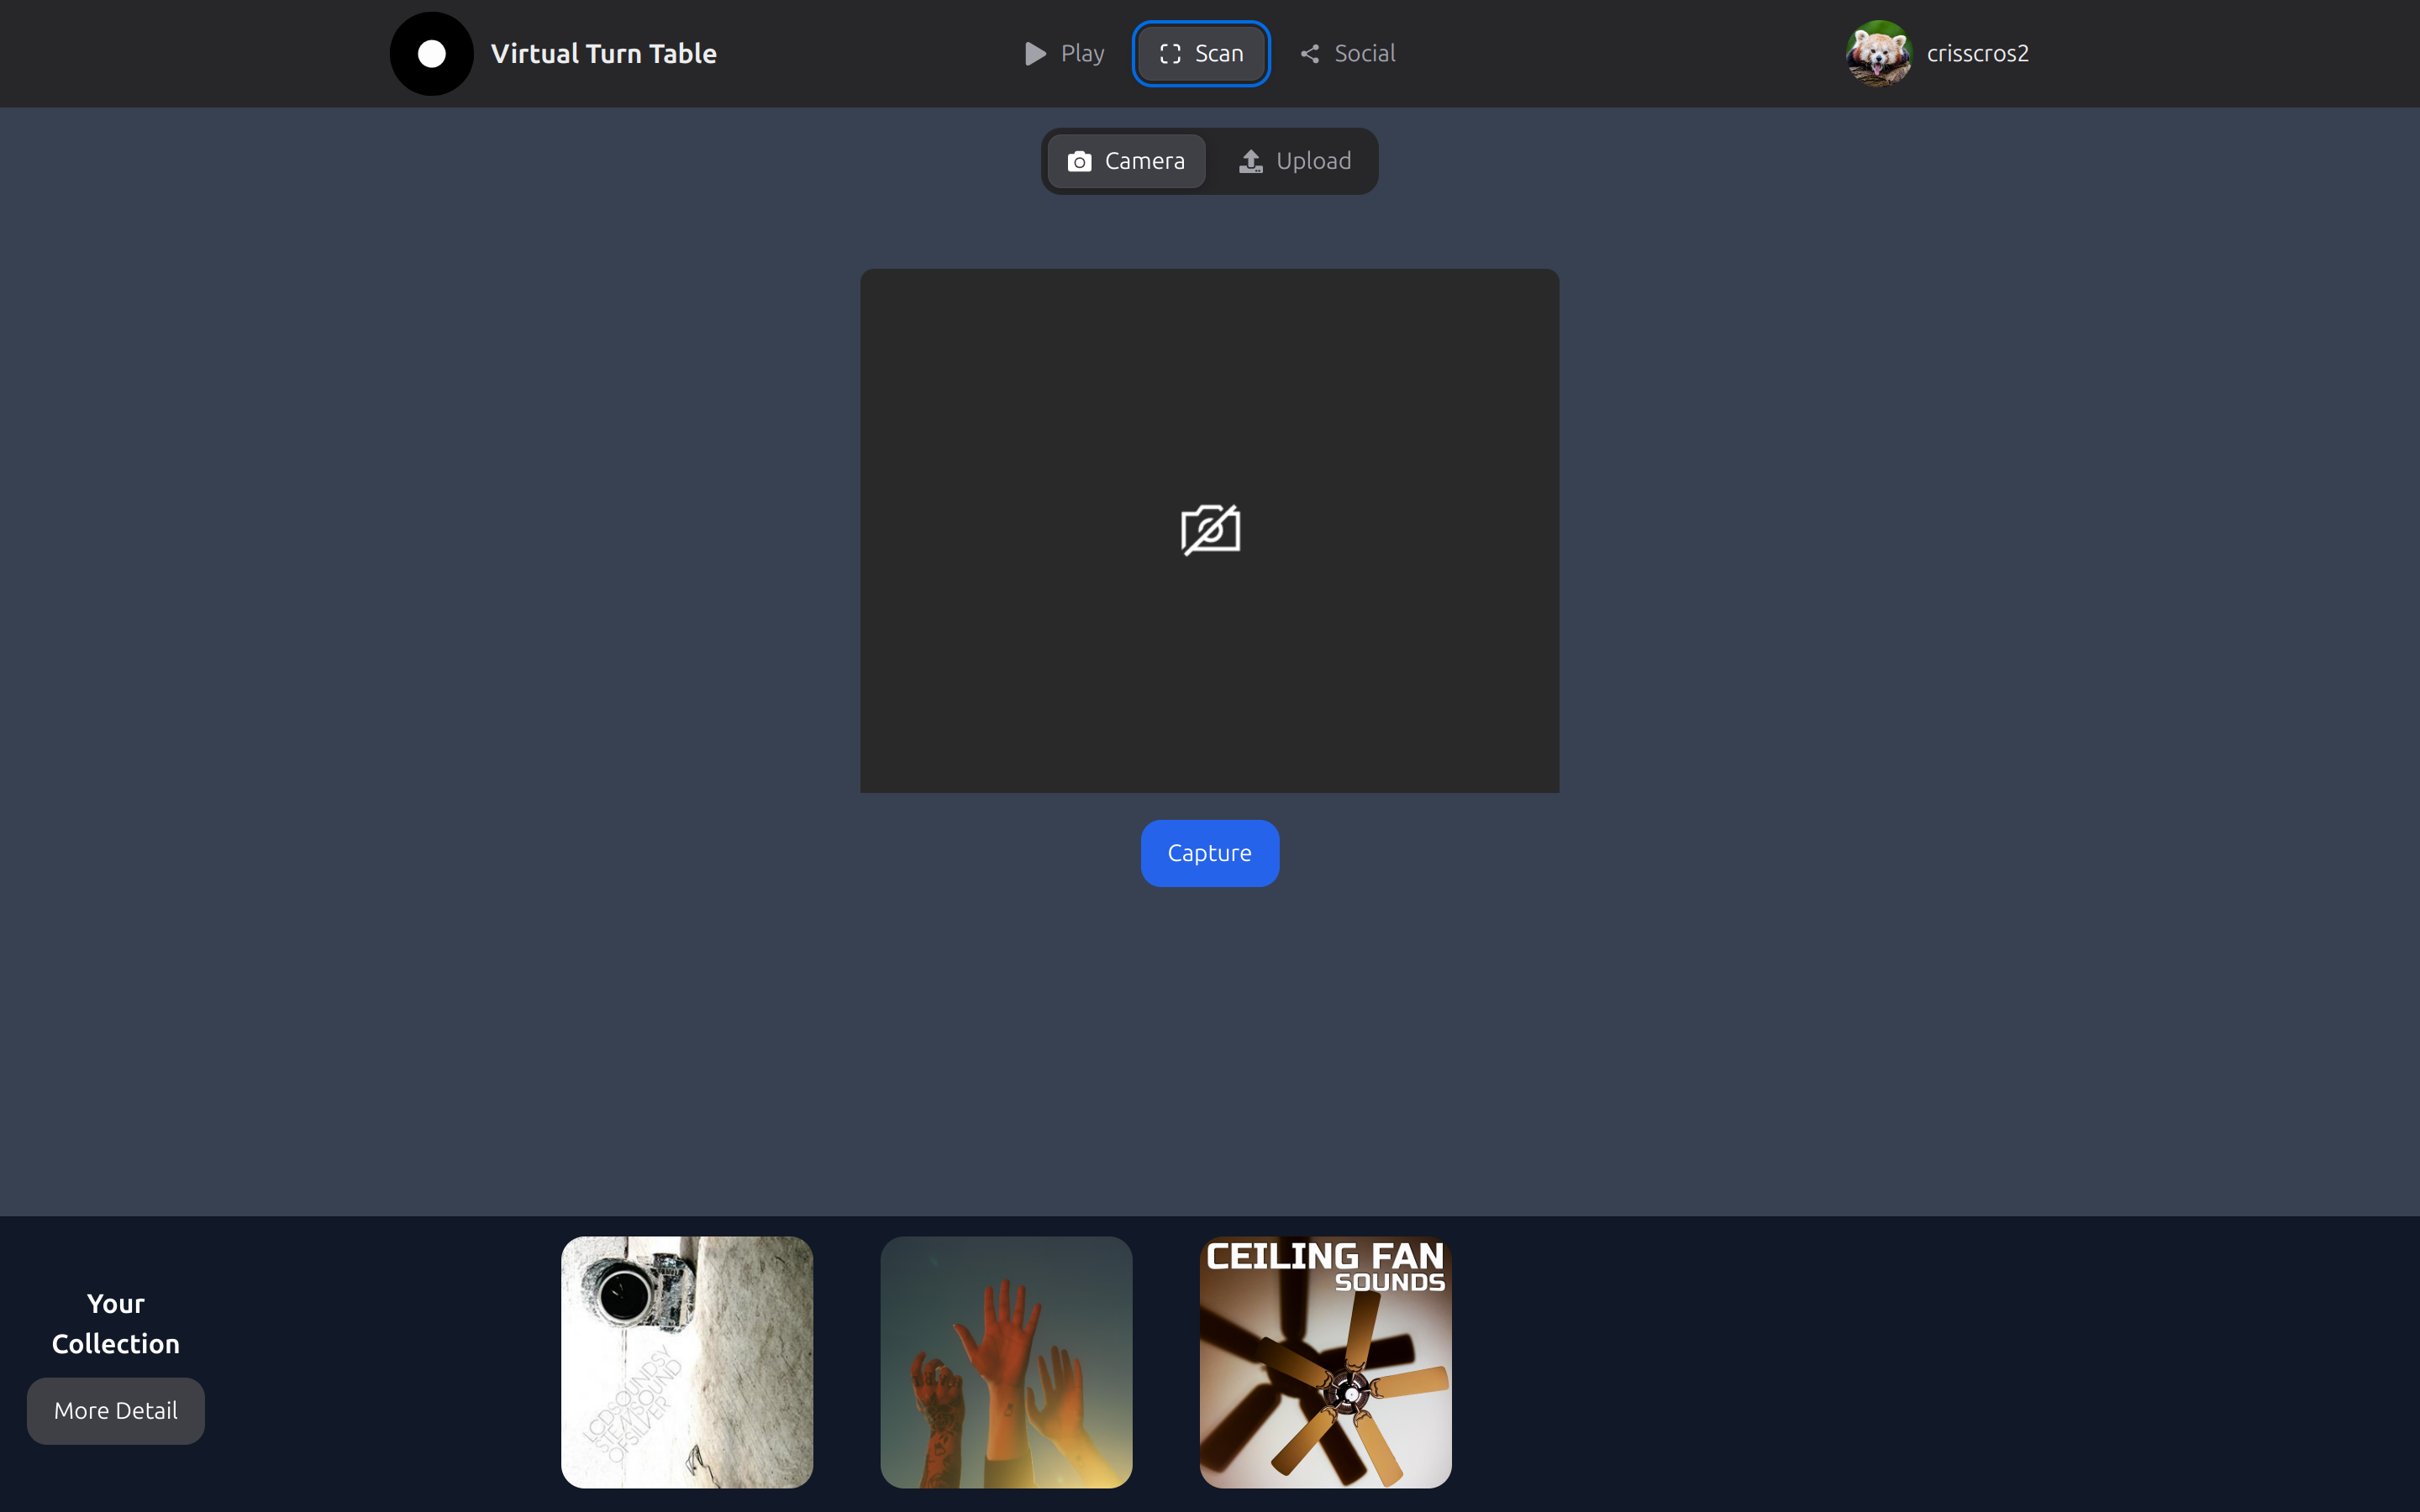
\includegraphics[width=0.8\textwidth]{figures/scan_screen.png}
    \caption{The scan screen of the application with the camera disabled}
    \label{fig:scan_screen}
\end{figure}

\subsubsection{Social Screen}
The social screen had the most changes from the design. It was originally implemented as shown in Figure~\ref{fig:social_screen_mockup}, but this proved to be too cluttered with larger collections being increasingly difficult to look through. The final design was inspired by the act of flicking through vinyl records in a record store. Each user's collection appears as a section of a grid where the albums in that collection pop up and down at random intervals. This allows for many more collections to be shown on the screen at once without overloading the user with information. The user can also load more collections by clicking the load more button at the bottom of the screen and view collections in more detail by clicking on them.

[TODO: Add Figure of the social screen]

\subsection{Automated Testing}
Automated testing of the frontend was done using Vitest a testing system built for projects using the Vite build system. A test driven development approach was taken so prior to starting the creation of each component a test case was written for each feature the component should have. Then the component was written that could pass those tests. In some cases the test cases found to not be perfect and so some refactoring was needed to make the tests pass. This was a good way to ensure that the components were built to the specification and that they could be tested in isolation.

The goal for the automated testing was to reach a coverage of 95\% which would provide certainty that the application was working as expected. To ensure this a GitHub action was set up to run the tests on every push to the repository and to fail the build if the coverage was below 95\% or if a build failed.

\subsection{Containerisation}
Containerisation for the frontend involved creating a Docker image which contained a built version of the frontend that on start would serve the application with an exposed port that users could connect to.

The building of the application was straightforward after dependencies are installed however these dependencies are not required to be in the Docker image once the build is complete and since cloud storage has a cost associated with it the size of the image should be minimised. To do this a two stage build is employed with the first stage being the build stage where the application is built and the second stage being the production stage where the built application is copied from the build stage and served.

\subsection{Dependency Management}
Dependencies for the front end were managed using Node Package Manager (NPM). As new dependencies were installed a file in the repository would be updated with the name of the package and the version. From this file anyone with NPM could install the dependencies by running a single command.

Automatic scanning of the dependencies file was done using Dependabot which would check for updates to the dependencies at a set interval, such as weekly or monthly, and create a pull request with the updates. This meant all dependencies were kept up to date and security vulnerabilities were patched as soon as possible whilst the automated tests allowed easy verification of if new dependency versions broke any functionality.

\subsection{Challenges}
\paragraph{Environment}
The biggest challenge in the frontend was managing environment variables. For different deployments of it different environment variables were needed. For example, the backend URL would be different for the development environment compared to the docker compose environment which would be different compared to the production environment. This issue was partially solved through the use of dotenv files which allowed environment variables to be defined in a file and then loaded into the application. However, these files could not be committed to git as they often contained secret keys for APIs and so had to be managed manually but once setup there were no issues.

\section{Backend}~\label{sec:backend-development}
\subsection{Implementation}
Each service was similar in its implementation, all consisting of a FastAPI application which would serve the API endpoints, and if needed WebSocket connections or database connections. They also all had two base endpoints which would be used for health checks and redirection to the documentation page, though this is removed from the deployed version of the application.

Each was split into routers which would categorise the endpoints into different sections, such as authentication or user endpoints. A list of all endpoints can be found in Appendix [TODO: Add appendix].

TODO: Add some more detail here

\subsubsection{BFF}
The BFF service was split into five routers; the music router, which contained all the endpoints related to playback and data about albums and songs; the user router, which contained all the endpoints related to user data; the image search router, which contained all the endpoints related to the image to album service; the authentication router, which contained all the endpoints related to authentication; and the social router, which contained all the endpoints related to the social functionality.

\subsubsection{User Data Service}
The user data service was the most complicated of the three services as it had to interact with a database. SQLAlchemy was used to interact with the database which meant each of the tables in the database had to be defined as a model in the code. The service was split into two routers; the user router, which contained all the endpoints related to specific users; and the social router, which contained all the endpoints related to social functionality.

A database migration tool was used to manage changes to the database schema to maintain data consistency. This tool would generate a migration file which could be run to update the database schema to match the new schema while keeping the data intact. Though during development this was not a problem as no real data was present in the database, it would be needed in a production environment as data must persist between updates even if the database schema changes.

\subsubsection{Image To Album Service}
The simplest of the three, the image to album service only consisted of two routers each with only one endpoint. The first router was for converting an image to some guess of an album and the second was for retrieving the Spotify album ID from the guess. This service was the most stateless of the three as it did not need to store any data between requests.

\subsubsection{Security}
For the user data and image to album services security was solved by adding middleware that would reject all requests not coming from the BFF service.

The BFF was more complicated as it had to receive calls from any user. To solve this a JSON Web Token (JWT) was used to authenticate the user. Once the user logs in with Spotify the frontend sends this to the backend where if it is valid a JWT is returned which can be sent in the header of requests to the BFF. The token can then be checked so that user can only access their own data and users without a token cannot access any data.

\subsection{Automated Testing}
Automated testing for the backend was done using the Pytest library which allowed the use of test fixtures to set up and tear down the environment for each test, such as database state. FastAPI provides a test client which can be used to call endpoints as if they were being called by a client.

Heavy use was made of mocking to simulated external API calls particularly in the BFF service which has to call the other two services. Without this it would be impossible to test each service in isolation.

\subsection{Containerisation}
Each of the three backend services were containerised in the same way using an Alpine Linux image with Python installed. Alpine was chosen as it is one of the smallest Linux distributions available, its lack of features would not be a problem as the services do not require any Linux features.

Unlike the frontend dependencies, the backend dependencies need to be present at runtime for the services to work, because of this a two stage build is not used. Instead, the dependencies are installed in the same stage as the application is copied into the image.

\subsection{Dependency Management}
Dependency management for Python is not standardised in the same way as it is for Node applications, there are different tools to manage dependencies such as Pipenv or Poetry. For simplicity the solution chosen was to use solely a requirements.txt file which lists all the dependencies for the project. The user can then install these dependencies with just pip, which is the most common package manager for Python.

Dependency updates were managed similarly to the frontend with Dependabot scanning the requirements.txt files and creating pull requests with updates to the dependencies. This was done at the same interval as the frontend, to ensure that the dependencies were kept up to date and security vulnerabilities were patched as soon as possible.

\section{Code Quality}~\label{sec:code-quality}
Code quality standards were maintained during development through the use of pre-commit hooks and GitHub actions. Pre-commit hooks were used to run linters and formatters on the code before it was committed to the repository. The benefit of doing this is that potentially bade code can be caught before it can even make it into the repository. This is extremely useful especially since during the development of this project there was only a single developer and so there was no code review process.

Automated tests and security scans were run every time a pull request was made to the repository as well as any commits pushed onto the main branch. This could have been integrated into the pre-commit hooks, but this was not done as the tests could take a long time to run and waiting for pre-commit hooks to complete would become a tedious process. Instead, the tests were run on the GitHub servers which could run the tests in parallel and so the time taken to run the tests was reduced.
